\documentclass[12pt,a4paper]{article}
\usepackage[utf8]{inputenc}
\usepackage{bold-extra}
\usepackage[pdfauthor={Luciano Henrique de Oliveira Santos}]{hyperref}
\usepackage[right=2.5cm,left=2.5cm,top=2cm,bottom=2cm]{geometry}
\usepackage{url}
\usepackage{graphicx}
\usepackage{float}
\usepackage{setspace}
\usepackage[export]{adjustbox}
\usepackage[usenames,dvipsnames]{xcolor}
\usepackage{listings}
\usepackage{textcomp}
\usepackage[]{algorithm2e}
\usepackage{tikz,forest}
\usetikzlibrary{arrows.meta}
\usepackage{datetime}
\newdateformat{monthyeardate}{%
  \monthname[\THEMONTH], \THEYEAR}

\renewcommand{\familydefault}{\sfdefault}

\title{Clue in Prolog\\{\Large -- A Didactic Example --}}
\author{Luciano Santos}
\date{\monthyeardate\today}

\newcommand{\varname}[1]{\texttt{#1}}
\newcommand{\varnameit}[1]{\textit{\texttt{#1}}}
\newcommand{\varnamebf}[1]{\textbf{\texttt{#1}}}
\newcommand{\varnamebfit}[1]{\textbf{\textit{\texttt{#1}}}}

\newcommand{\predprot}[2]{{\color{MidnightBlue}\varnamebf{#1}}/{\color{Mulberry}\varname{#2}}}
\newcommand{\predname}[1]{{\color{MidnightBlue}\varname{#1}}}
\newcommand{\And}{\textbf{and}}
\newcommand{\Not}{\textbf{not}}

\newtheorem{definition}{Definition}[section]
\newtheorem{constraint}{Constraint}[section]


% --- ugly internals for language definition ---
% see: http://tex.stackexchange.com/questions/161235/can-the-listings-package-be-set-up-to-highlight-prolog-code-like-minted-does
%
\makeatletter

\newcommand\PrologPredicateStyle{}
\newcommand\PrologVarStyle{}
\newcommand\PrologAnonymVarStyle{}
\newcommand\PrologOpStyle{}
\newcommand\PrologAtomStyle{}
\newcommand\PrologOtherStyle{}
\newcommand\PrologCommentStyle{}


% useful switches (to keep track of context)

\newif\ifpredicate@prolog@
\newif\ifwithinparens@prolog@

% save definition of underscore for test
\lst@SaveOutputDef{`_}\underscore@prolog

% local variables
\newcount\currentchar@prolog

\newcommand\@testChar@prolog%
{%
  % if we're in processing mode...
  \ifnum\lst@mode=\lst@Pmode%
    \detectTypeAndHighlight@prolog%
  \else
    % ... or within parentheses
    \ifwithinparens@prolog@%
      \detectTypeAndHighlight@prolog%
    \fi
  \fi
  % Some housekeeping...
  \global\predicate@prolog@false%
}

% helper macros
\newcommand\detectTypeAndHighlight@prolog
{%
  % First, assume that we have an atom.
  \def\lst@thestyle{\PrologAtomStyle}%
  % Test whether we have a predicate and modify the style accordingly.
  \ifpredicate@prolog@%
    \def\lst@thestyle{\PrologPredicateStyle}%
  \else
    % Test whether we have a predicate and modify the style accordingly.
    \expandafter\splitfirstchar@prolog\expandafter{\the\lst@token}%
    % Check whether the identifier starts by an underscore.
    \expandafter\ifx\@testChar@prolog\underscore@prolog%
      % Check whether the identifier is '_' (anonymous variable)
      \ifnum\lst@length=1%
        \let\lst@thestyle\PrologAnonymVarStyle%
      \else
        \let\lst@thestyle\PrologVarStyle%
      \fi
    \else
      % Check whether the identifier starts by a capital letter.
      \currentchar@prolog=65
      \loop
        \expandafter\ifnum\expandafter`\@testChar@prolog=\currentchar@prolog%
          \let\lst@thestyle\PrologVarStyle%
          \let\iterate\relax
        \fi
        \advance \currentchar@prolog by 1
        \unless\ifnum\currentchar@prolog>90
      \repeat
    \fi
  \fi
}
\newcommand\splitfirstchar@prolog{}
\def\splitfirstchar@prolog#1{\@splitfirstchar@prolog#1\relax}
\newcommand\@splitfirstchar@prolog{}
\def\@splitfirstchar@prolog#1#2\relax{\def\@testChar@prolog{#1}}

% helper macro for () delimiters
\def\beginlstdelim#1#2%
{%
  \def\endlstdelim{\PrologOtherStyle #2\egroup}%
  {\PrologOtherStyle #1}%
  \global\predicate@prolog@false%
  \withinparens@prolog@true%
  \bgroup\aftergroup\endlstdelim%
}

% language name
\newcommand\lang@prolog{Prolog-pretty}
% ``normalised'' language name
\expandafter\lst@NormedDef\expandafter\normlang@prolog%
  \expandafter{\lang@prolog}

% language definition
\expandafter\expandafter\expandafter\lstdefinelanguage\expandafter%
{\lang@prolog}
{%
  language            = Prolog,
  keywords            = {},      % reset all preset keywords
  showstringspaces    = false,
  alsoletter          = (,
  alsoother           = @$,
  moredelim           = **[is][\beginlstdelim{(}{)}]{(}{)},
  MoreSelectCharTable =
    \lst@DefSaveDef{`(}\opparen@prolog{\global\predicate@prolog@true\opparen@prolog},
}

% Hooking into listings to test each ``identifier''
\newcommand\@ddedToOutput@prolog\relax
\lst@AddToHook{Output}{\@ddedToOutput@prolog}

\lst@AddToHook{PreInit}
{%
  \ifx\lst@language\normlang@prolog%
    \let\@ddedToOutput@prolog\@testChar@prolog%
  \fi
}

\lst@AddToHook{DeInit}{\renewcommand\@ddedToOutput@prolog{}}

\makeatother
%
% --- end of ugly internals ---


% redefinition of user macros for Prolog style
\renewcommand\PrologPredicateStyle{\color{MidnightBlue}}
\renewcommand\PrologVarStyle{\color{ForestGreen}}
\renewcommand\PrologAnonymVarStyle{\color{Magenta}}
\renewcommand\PrologOpStyle{\color{Magenta}}
\renewcommand\PrologAtomStyle{\color{YellowOrange}}
\renewcommand\PrologCommentStyle{\itshape\color{Gray}}
\renewcommand\PrologOtherStyle{\color{Black}}

% custom style definition
\lstdefinestyle{Prolog-pygsty}{
  language     = Prolog-pretty,
  upquote      = true,
  stringstyle  = \PrologAtomStyle,
  commentstyle = \PrologCommentStyle,
  literate     =
    {:-}{{\PrologOpStyle :- }}2
    {,}{{\PrologOtherStyle ,}}1
    {.}{{\PrologOtherStyle .}}1
    {0}{{{\PrologAtomStyle{0}}}}1
    {1}{{{\PrologAtomStyle{1}}}}1
    {2}{{{\PrologAtomStyle{2}}}}1
    {3}{{{\PrologAtomStyle{3}}}}1
    {4}{{{\PrologAtomStyle{4}}}}1
    {5}{{{\PrologAtomStyle{5}}}}1
    {6}{{{\PrologAtomStyle{6}}}}1
    {7}{{{\PrologAtomStyle{7}}}}1
    {8}{{{\PrologAtomStyle{8}}}}1
    {9}{{{\PrologAtomStyle{9}}}}1
}


\lstset{
}

% global settings
\lstset{
  captionpos = below,
  frame      = single,
  columns    = fullflexible,
  basicstyle = \scriptsize\ttfamily,
}


\begin{document}

\maketitle

\section{Introduction}

This is the documentation for a simple script in SWI-Prolog that plays the game Clue\footnote{\url{http://www.hasbro.com/en-us/toys-games/hasbro-games:clue} (accessed on August, 2016)}. This implementation follows a didactic approach, not aimed at creating an advanced AI system that employs complex strategies and human behaviour models to master the game. It simply illustrates how a declarative language can be used to play a relatively simple game based on a certain set of rules.

The implementation is based on the rules for the 2002 version of the game (see PDF on the root folder) and the board on Figure \ref{fig:board}.

\begin{figure}[H]
	\centering
	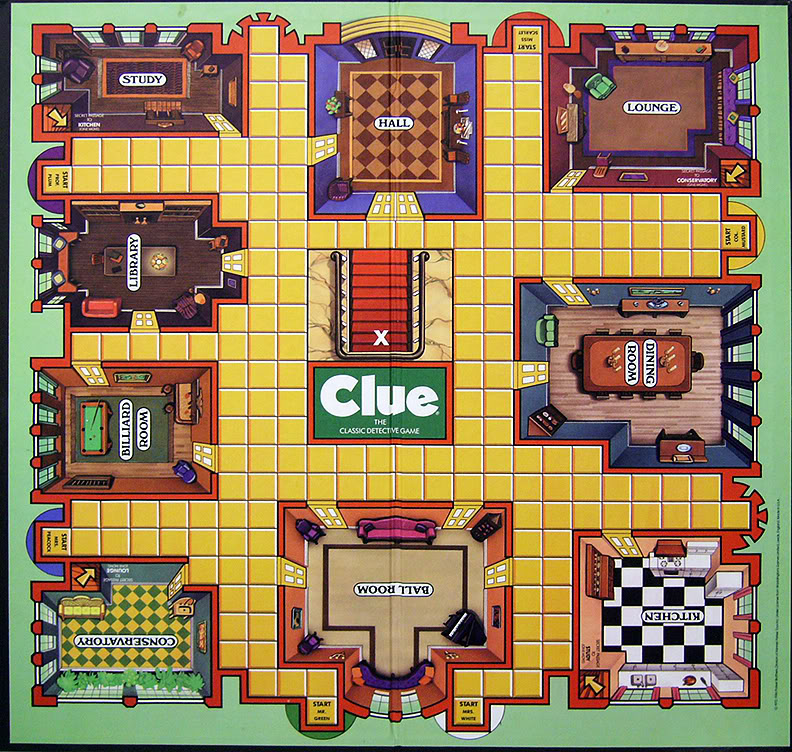
\includegraphics[width=0.5\textwidth]{board.jpg}
	\caption{The game board.}
	\label{fig:board}
\end{figure}

The following principles were observed in this implementation to make it simple:
\begin{itemize}
    \item no long-term planning -- for each action and information received, the agent updates its 'knowledge base' and, on each turn, it makes an independent decision based on the current knowledge, instead of following a planned route;
    
    \item no lucky guesses -- the agent only makes an accusation if it's certain that it's true;
    
    \item no poker face -- the agent only acts to acquire more information, and will not make a move or guess for the sole purpose of misleading other players;
    
    \item no mind reading -- the agent will not infer information from other players actions, except facts that can be logically proven; it will not try to predict how people would or should behave, however, it will assume that everyone will play strategically, \textit{e.g.}, if the player to the left has already shown a certain card before, that card will not be used on a next guess, because a smart player would keep showing the same card over and over again, even if she had a different one to show.
\end{itemize}

The sections below describe the rationale and the details of this implementation. Section \ref{sec:board} shows how the game board and the current position of each player is stored internally and how the agent finds the shortest path to a given goal. Section \ref{sec:decisions} describes how the knowledge acquired as the match progresses is represented, and how the game decides the action to take in each turn. Finally, Section \ref{sec:interface} explains the predicates that allow the final user to initialize and subsequently interact with the agent.

\section{Moving on the Board}
\label{sec:board}

The game board is seen internally as a grid of size $24\times25$. As illustrated by Figure \ref{fig:board-grid}, coordinates are relative to the lower left corner, and start on $0$.

\begin{figure}[H]
	\centering
	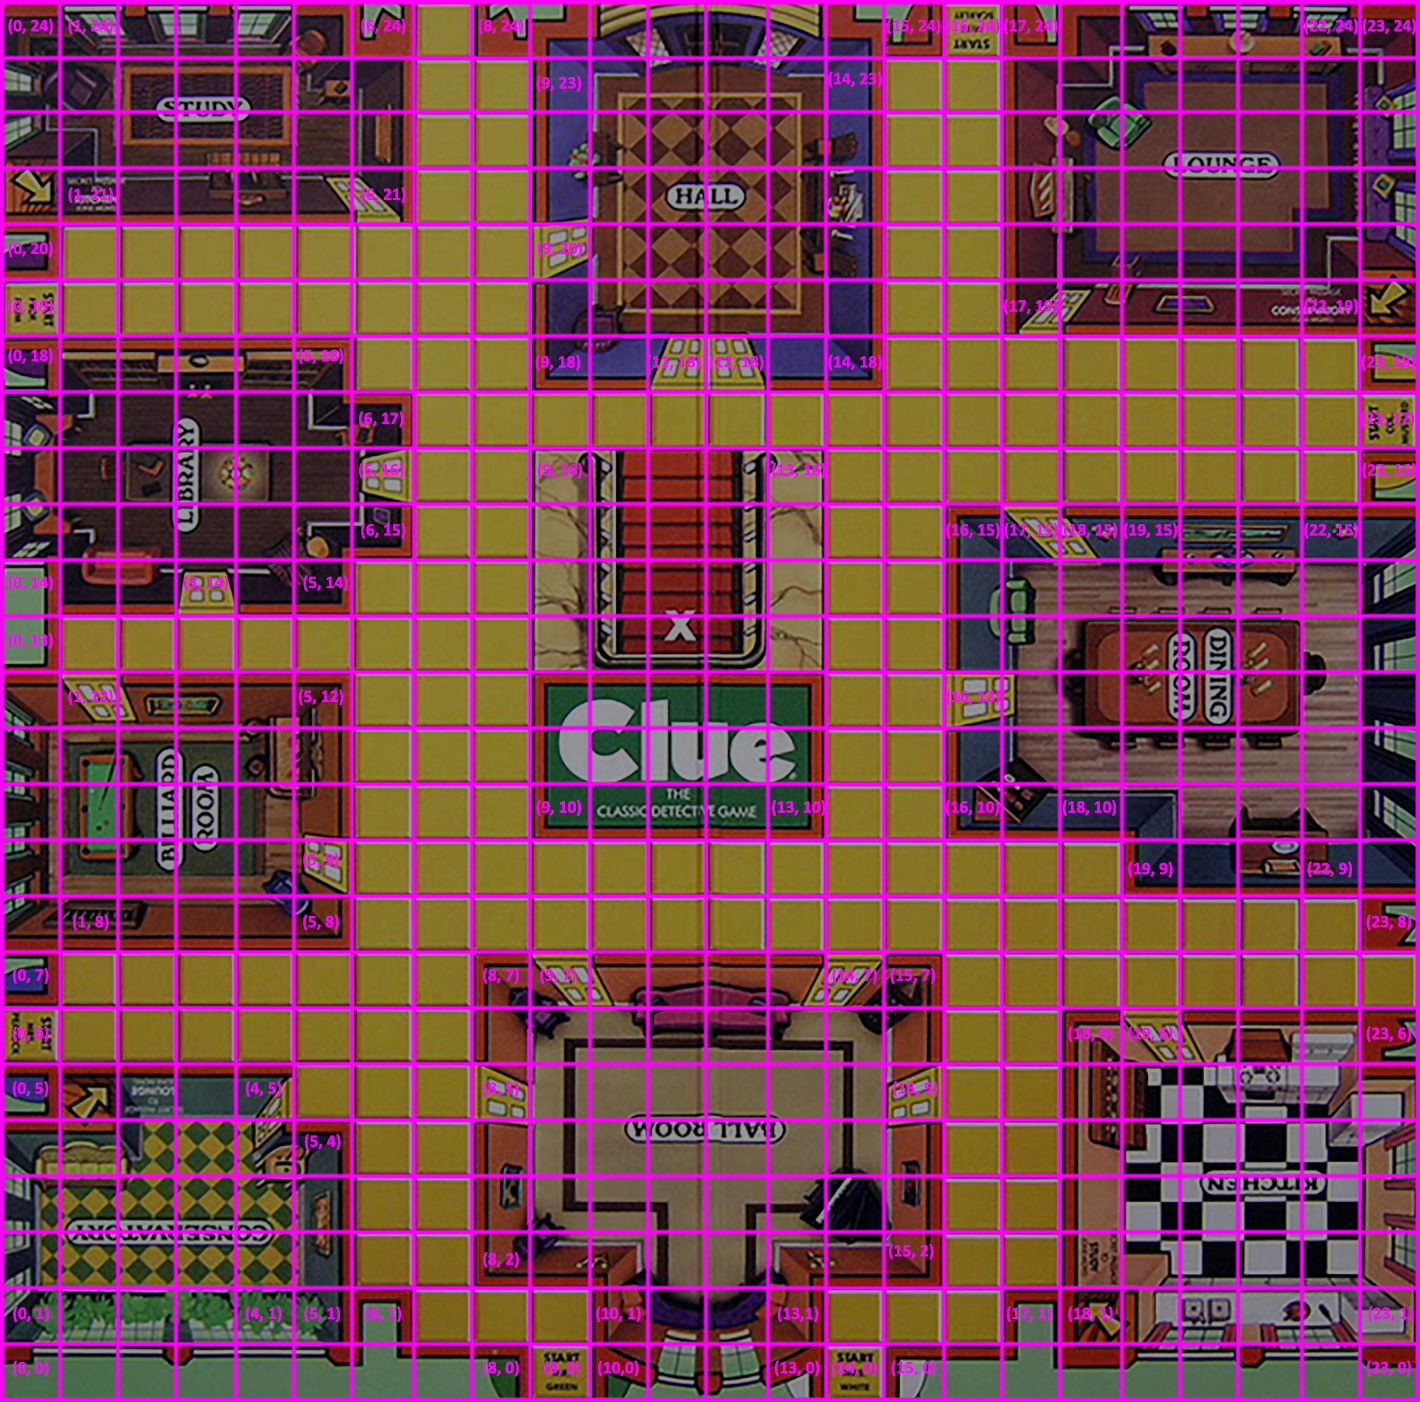
\includegraphics[width=0.95\textwidth]{board-grid.png}
	\caption{The game board.}
	\label{fig:board-grid}
\end{figure}

\subsection{Constraints}

The following predicates describe the constraints that affect movements inside the board:
\begin{itemize}
    \item \predprot{blocked}{1} -- is true for the tuple \varname{(X, Y)} if it represents a location that is blocked, \textit{i.e.}, it's inside a room or in a wall;
    
    \item \predprot{door}{2} -- is true for the tuple \varname{(X, Y)} and room \varname{R} if it's possible to enter R from \varname{(X, Y)};
    
    \item \predprot{passage}{2} -- is true for arguments \varname{Source}, \varname{Dest} if there is a secret passage from room \varname{Source} to room \varname{Dest};
    
    \item \predprot{position}{2} (\textit{dynamic}) -- is true for the tuple \varname{(X, Y)} and character \varname{C} if \varname{(X, Y)} is the current position of \varname{C} on the board;
\end{itemize}

Based on the game rules, once inside the room, the position of the individual cell occupied by the player is irrelevant, it's as if each room is a ``supercell''. For that reason, it's only necessary to know if the player is inside a room and, if not, in which (free) cell she is. Also, because each room is accessible only from specific cells, and each of these cells gives access to one, and only one room, it's unnecessary to know if a given cell belongs to a specific room or wall, it's only important to know which are the access cells (\textit{i.e.}, doors) to which room, and if a given cell is free or not.

Since the blocked areas are more ``regular'', \textit{i.e.}, they are more easily described in terms of rectangles, it was a design choice to use a predicate \predname{blocked} that defines if a certain position is blocked or not. The same end could be achieved with an opposite predicate \predname{free}. Figure \ref{fig:blocked} shows the (static) declaration of the blocked cells in the board.

The predicate \predname{door} says if a cell is an access cell, and to which room it gives access to. Since entering the room doesn't count as a step, it's enough to reach these access cells when finding a path and then switching the state to ``inside the room''. Figure \ref{fig:door} shows the (static) declaration of all the doors in the game.

The predicate \predname{passage} is a special case, to represent the information that there are secret passages between the rooms in the (opposite) corners of the board. As shown in Figure \ref{fig:passage}, it is implemented as a commutative operation by using an auxiliary predicate.

Finally, the predicates \predname{position} and \predname{last\_position} (this one will be used later) inform the current and the last turn's position of a player, respectively. For any atom \varname{n} that is a valid player name, there will be exactly one fact that says ``the position of \varname{n} is \varname{(X, Y)}''. The agent makes sure this holds true by defining the start position shown on the board once (Figure \ref{fig:start-positions}), and \textit{retracting} and \textit{asserting} that position any time a player's position changes, as will be explained on Section \ref{sec:decisions}. When a player enters a room, her position becomes that room's name.

Other constraints, such as the board boundaries, are checked on the path finding algorithm, as described on the next section.

\subsection{Path Finding}

One of the key actions the agent must perform is movement. The first step necessary to move on the board is to answer the question: ``where can I go from my current position?''. If the player is in a cell adjacent to a door, she can enter the room; if she is in a corner room, she could use a secret passage. However, to get to the point where she could enter a room, the player must first reach a door, and using a secret passage is a trivial action. Thus, right now, only the problem of moving from a free cell to another free cell will be addressed. In order to solve that problem, the agent must determine the shortest path between two points.

As the game rules state, if the player is currently in any given cell, she can only move to another empty cell vertically or horizontally. To express that relationship, the predicate \predprot{neighbor}{2} is defined (Figure \ref{fig:neighbor}). It will be true for points \varname{(Xs, Ys)}, \varname{(Xn, Yn)} if \varname{(Xn, Yn)} is exactly one cell away from \varname{(Xs, Ys)}, moving either vertically or horizontally (but not both).

\begin{figure}[H]
	\centering
\begin{lstlisting}[style=Prolog-pygsty]
%% neighbor((Xs, Ys), (Xn, Yn)) - <Xn, Yn> is neighbor of <Xs, Ys>.
neighbor((Xs, Ys), (Right, Ys)) :- Right is Xs + 1.
neighbor((Xs, Ys), (Left, Ys)) :- Left is Xs - 1.
neighbor((Xs, Ys), (Xs, Up)) :- Up is Ys + 1.
neighbor((Xs, Ys), (Xs, Down)) :- Down is Ys - 1.
\end{lstlisting}
	\caption{The declaration of the predicate \predname{neighbor}.} 
	\label{fig:neighbor}
\end{figure}

Now, besides checking if a certain cell is a neighbor, it must also be possible to actually move there, \textit{i.e.}, it must be inside the boundaries of the board and not occupied by any other player or blocked, as previously defined. All theses cases are summarized by the predicate \predprot{is\_free}{1}, shown in Figure \ref{fig:is-free}.

\begin{figure}[H]
	\centering
\begin{lstlisting}[style=Prolog-pygsty]
%% is_free((X, Y)) - the position <X, Y> can bee occupied by a character.
is_free((X, Y)) :-
		X >= 0, X =< 23, Y >= 0, Y =< 24, % inside the board
		\+ position((X, Y), _), % not currently occupied by anyone
		\+ blocked((X, Y)). % not a room or a wall
\end{lstlisting}
	\caption{The declaration of the predicate \predname{is\_free}.} 
	\label{fig:is-free}
\end{figure}

Once all the constraints on movement between two adjacent cells have been represented, it's possible to implement the algorithm to find the shortest path between two points on the map, if such a path exists. More precisely, the algorithm here implemented finds the shortest path between a given free cell \varname{(Xs, Ys)} and the closest door. Subsequent backtracking on the predicate will return all the doors of the board, ascendingly ordered by path length.

The simplest way to tackle this task is using BFS (Breadth-first Search). The idea is simple: inspect the source node; then all the nodes exactly 1 step away from the source node; then all the nodes exactly 2 steps away from the source node; and so on. This ensures that, if a path exists, it will be found and will be a shortest path. If the backtracking mechanism continues from the state where it found a path, the next door found will have the next shortest path.

To make sure that the nodes are inspected in the correct order, a queue is used. This queue begins with the source node. At each iteration, the node at the head of the queue is removed and inspected. If it's not a door, then its adjacent nodes are enqueued and the search continues. To prevent the search from recursing infinitely, it's necessary to keep a set of all nodes seen so far, so only adjacent nodes not yet inspected are enqueued.

Notice that this algorithm and the way the constraints are defined respect the game rules that state \textit{``you must not enter or land on a square that's already occupied''}, \textit{``you may not [...] enter the same square twice on the same turn''}, \textit{``you may not pass through a door that's blocked by an opponent's character''} and \textit{``when you pass through a door, do not count the doorway itself as space''}. This derives from the facts that every player's positions are considered blocked cells, that BFS never moves to a previously seen cell and that doors are represented by the only cell that gives access to them, and it's necessary and sufficient to reach them to enter a room.

The code for this search algorithm is shown in Figure \ref{fig:bfs}. The predicate \predprot{closest\_door}{3} receives a source point and unifies the name of the room with the closest door and the path to that door as a list of points. This predicate itself only sets up the initial values for the algorithm -- the queue and the ``seen nodes'' set are both initialized to a unitary list containing the source point -- and calls the auxiliary predicate \predprot{closets\_door\_aux}{4} to actually perform the search.

The base case for this predicate is when the head of the queue is a door. If that happens, it will unify to the found door's room and the path is a unitary list containing just the door. The recursive step will extract the head of the queue, enqueue all adjacent cells that are free and have not yet been seen (described by \predprot{valid\_adjacent}{3}), mark all the neighbor cells are seen, and recursively continue walking on the list. As the recursive calls return, the path is built by inserting the inspected node on the head of the result list.

\begin{figure}[H]
	\centering
\begin{lstlisting}[style=Prolog-pygsty]
%% closest_door((Xs, Ys), Room, Path) - starting at <Xs, Ys>, finds
%% the closest Room door and the Path to it
unseen_neighbor((X, Y), (Xd, Yd), Seen) :-
		neighbor((X, Y), (Xd, Yd)),
		\+ member((Xd, Yd), Seen).
valid_adjacent((X, Y), (Xd, Yd), Seen) :-
		unseen_neighbor((X, Y), (Xd, Yd), Seen),
		is_free((Xd, Yd)).
closest_door_aux(Room, [Head], [Head|_], _) :- door(Head, Room).
closest_door_aux(Room, [(X, Y)|PTail], [(X, Y)|QTail], Seen) :-
		% enqueues all non-seen adjacents to which it's possible to move
		findall((Xd, Yd), valid_adjacent((X, Y), (Xd, Yd), Seen), ValidAdjacents),
		append(QTail, ValidAdjacents, NewQueue),
		% stores all adjacent nodes as seen, to cut the search recursion
		findall((Xa, Ya), unseen_neighbor((X, Y), (Xa, Ya), Seen), Neighbors),
		append(Neighbors, Seen, NewSeen),
		closest_door_aux(Room, PTail, NewQueue, NewSeen). % recursive definition
closest_door((Xs, Ys), Room, Path) :-
		closest_door_aux(Room, Path, [(Xs, Ys)], [(Xs, Ys)]).
\end{lstlisting}
	\caption{The breadth-first search used to find the closest door, given a source cell.} 
	\label{fig:bfs}
\end{figure}

Even though this algorithm finds the path between two cells on the board, the agent actually needs to solve the more general problem of finding the closest doors when departing from multiple source cells. That's because, if the agent is inside a room, there could be multiple exits to choose from, thus, it should find the best option taking into account all these exits.

The na\"{i}ve approach would be to find lists with all the paths for each exit, merge these lists while ordering the elements (paths) by length and, finally, traverse the result. However, that solution is both inefficient and \textit{imperative}, in the sense that it tells the steps to solve the problem, instead of taking advantage of the declarative paradigm.

What happens if the queue in the previous solution is initialized with multiple source cells, instead of just one?
\begin{itemize}
    \item when the first element of the queue is inspected, all its adjacent nodes will be enqueued \textbf{after} all the other sources, which are currently on the queue (as long as those adjacent nodes aren't sources themselves);
    
    \item when the next element is inspected (another source), once again, all its \textit{not already on the queue} adjacents will also be enqueued;
    
    \item after all the sources nodes are inspected first, the next element to be inspected is exactly one step away from one of the sources; actually, all the elements that are exactly one step away from at least one of the sources will be inspected next, and their adjcent nodes will be enqueued;
    
    \item by analogy, all the elements that are exactly two steps away from \textbf{at least one} of the sources will be analyzed next, and so on...
\end{itemize}

Ergo, it's possible to conclude that, just by initializing the queue with the multiple sources, the order in which the elements are inspected still ensures that doors are searched \textit{breadth-first} and, as a consequence, the doors are found in order, from the closest to the farthest, only now the distance applies to any one of the possible sources.

There's one problem though: in the previous algorithm, since there was only one source, the path could be rebuilt implicitly within the backtracking mechanism. The base of the recursion was the door, and the recursive steps would attach one cell to the head of the resulting list, until the caller of the predicate would have the whole path ready. With multiple sources, however, it's necessary to explicitly store, for each cell that is reached, that cell's parent, \textit{i.e.}, the cell \textit{from which} it was reached.

\begin{figure}[H]
	\centering
\begin{lstlisting}[style=Prolog-pygsty]
%% closest_door((Xs, Ys), Room, Path) - starting at <Xs, Ys>, finds
%% the closest Room door and the Path to it
unseen_neighbor((X, Y), (Xd, Yd), Seen) :-
		neighbor((X, Y), (Xd, Yd)),
		\+ member(((Xd, Yd), _), Seen).
valid_adjacent((X, Y), (Xd, Yd), Seen) :-
		unseen_neighbor((X, Y), (Xd, Yd), Seen),
		is_free((Xd, Yd)).
add_parent([], _, []).
add_parent([Node|NodesTail], Parent, [(Node, Parent)|LinkedTail]) :-
		add_parent(NodesTail, Parent, LinkedTail).
build_path(Head, Seen, [Head]) :- member((Head, nil), Seen).
build_path(Head, Seen, [Head|Tail]) :-
		member((Head, Parent), Seen),
		build_path(Parent, Seen, Tail).
closest_door_aux(Room, Path, [Head|_], Seen) :-
		door(Head, Room),
		build_path(Head, Seen, InversePath),
		reverse(InversePath, Path),
		print(Path),nl.
closest_door_aux(Room, Path, [(X, Y)|QTail], Seen) :-
		% enqueues all non-seen adjacents to which it's possible to move
		findall((Xd, Yd), valid_adjacent((X, Y), (Xd, Yd), Seen), ValidAdjacents),
		append(QTail, ValidAdjacents, NewQueue),
		% stores all adjacent nodes as seen, to cut the search recursion
		findall((Xa, Ya), unseen_neighbor((X, Y), (Xa, Ya), Seen), Neighbors),
		add_parent(Neighbors, (X, Y), LinkedNeighbors),
		append(LinkedNeighbors, Seen, NewSeen),
		closest_door_aux(Room, Path, NewQueue, NewSeen). % recursive definition
closest_door((Xs, Ys), Room, Path) :-
		closest_door_aux(Room, Path, [(Xs, Ys)], [((Xs, Ys), nil)]).
closest_door(SourceRoom, TargetRoom, Path) :-
		valid_rooms(ValidRooms), member(SourceRoom, ValidRooms),
		findall(Exit, door(Exit, SourceRoom), Exits),
		add_parent(Exits, nil, LinkedExits),
		closest_door_aux(TargetRoom, Path, Exits, LinkedExits).
\end{lstlisting}
	\caption{The breadth-first search used to find the closest door, given multiple source cells.} 
	\label{fig:bfs-ms}
\end{figure}

Figure \ref{fig:bfs-ms} shows the new version of the algorithm that includes these changes. Now, the \varname{Seen} set elements are tuples \varname{(Cell, Parent)} that store not only the coordinate of the cells that were already seen, but also their parent (which can be the coordinates of a previously seen cell or \varname{nil} for the source cells). All predicates were updated to handle this new representation.

The auxiliary predicate \predprot{add\_parent}{3} simply receives a list \varname{Nodes} and an element \varname{Parent} and generates a new list with each element \varname{N} of \varname{Nodes} in a tuple \varname{(N, Parent)}.

Finally, the new recursive predicate \predprot{build\_path}{3} is used to explicitly rebuild the path when a door is reached, given the set of seen nodes (and their parents). The predicate inspects the \varname{Head} element using the \varname{Seen} set and generates the \varname{Path} as a list; the base case happens when the parent of \varname{Head} is \varname{nil}, which generates the unitary list; the recursive case adds \varname{Head} to the list and inspects its non-nil parent. Since this predicate is called when a door is found, the path is actually generated in the reverse order, so the resulting list is reversed before being returned to the original caller.


\begin{figure}[H]
	\centering
\begin{lstlisting}[style=Prolog-pygsty]
%% blocked((X, Y)) - point <X, Y> is inside a room or is a wall
% conservatory
blocked((X, Y)) :- Y =:= 0, X >= 0, X =< 8.
blocked((X, Y)) :- X >= 0, X =< 4, Y >= 1, Y =< 5.
blocked((X, Y)) :- X =:= 5, Y >= 1, Y =< 4.
blocked((6, 1)).
% ball room
blocked((X, Y)) :- X >= 10, X =< 13, Y >= 0, Y =< 1.
blocked((X, Y)) :- X >= 8, X =< 15, Y >= 2, Y =< 7.
% kitchen
blocked((X, Y)) :- Y =:= 0, X >= 15, X =< 23.
blocked((17, 1)).
blocked((X, Y)) :- X >= 18, X =< 23, Y >= 1, Y =< 6.
% dining room
blocked((X, Y)) :- X >= 16, X =< 18, Y >= 10, Y =< 15.
blocked((X, Y)) :- X >= 19, X =< 22, Y >= 9, Y =< 15.
blocked((X, Y)) :- X =:= 23, Y >= 8, Y =< 16.
% lounge
blocked((X, Y)) :- X >= 17, X =< 22, Y >= 19, Y =< 24.
blocked((X, Y)) :- X =:= 23, Y >= 18, Y =< 24.
% hall
blocked((X, Y)) :- X >= 9, X =< 14, Y >= 18, Y =< 23.
blocked((X, Y)) :- Y =:= 24, X >= 8, X =< 15.
% study
blocked((X, Y)) :- X =:= 0, Y >= 20, Y =< 24.
blocked((X, Y)) :- X >= 1, X =< 6, Y >= 21, Y =< 24.
% library
blocked((X, Y)) :- X >= 0, X =< 5, Y >= 14, Y =< 18.
blocked((X, Y)) :- X =:= 6, Y >= 15, Y =< 17.
% billiard room
blocked((X, Y)) :- X =:= 0, Y >= 7, Y =< 13.
blocked((X, Y)) :- X >= 1, X =< 5, Y >= 8, Y =< 12.
% stairs
blocked((X, Y)) :- X >= 9, X =< 13, Y >= 10, Y =< 16.
\end{lstlisting}
	\caption{The declaration of the predicate \predname{blocked}.} 
	\label{fig:blocked}
\end{figure}

\begin{figure}[H]
	\centering
\begin{lstlisting}[style=Prolog-pygsty]
%% door((X, Y), R) - there's a door to room R from point <X, Y>
door((5, 5), 'conservatory').
door((7, 5), 'ball room').
door((16, 5), 'ball room').
door((9, 8), 'ball room').
door((14, 8), 'ball room').
door((19, 7), 'kitchen').
door((15, 12), 'dining room').
door((17, 16), 'dining room').
door((17, 18), 'lounge').
door((8, 20), 'hall').
door((11, 17), 'hall').
door((12, 17), 'hall').
door((6, 20), 'study').
door((3, 13), 'library').
door((7, 16), 'library').
door((1, 13), 'billiard room').
door((6, 9), 'billiard room').
\end{lstlisting}
	\caption{The declaration of the predicate \predname{door}.} 
	\label{fig:door}
\end{figure}

\begin{figure}[H]
	\centering
\begin{lstlisting}[style=Prolog-pygsty]
%% passage(Src, Dst) - there's a passage from Src to Dst
passage_aux('conservatory', 'lounge').
passage_aux('kitchen', 'study').
passage(Src, Dst) :- passage_aux(Src, Dst) ; passage_aux(Dst, Src).
\end{lstlisting}
	\caption{The declaration of the predicate \predname{passage}.} 
	\label{fig:passage}
\end{figure}

\begin{figure}[H]
	\centering
\begin{lstlisting}[style=Prolog-pygsty]
%% position((X, Y), C) - the current position of character C is <X, Y>
%% here, it's initialized to the start position at the board.
%% this predicate will be "rewritten" whenever the script's own
%% character moves or it receives information that another character
%% moved.
:- dynamic position/2.
position((16, 24), 'scarlet').
position((23, 17), 'mustard').
position((14, 0), 'white').
position((9, 0), 'green').
position((0, 6), 'peacock').
position((0, 19), 'plum').

%% last_position((X, Y), C) - the position of character C was <X, Y> last turn.
%% it'll be updated as the script's own character moves or it receives
%% information that another character moved.
:- dynamic last_position/2.
last_position(nil, 'scarlet').
last_position(nil, 'mustard').
last_position(nil, 'white').
last_position(nil, 'green').
last_position(nil, 'peacock').
last_position(nil, 'plum').
\end{lstlisting}
	\caption{The declaration of the predicate \predname{position} and the initial position of all players.} 
	\label{fig:start-positions}
\end{figure}

\section{Making Decisions}
\label{sec:decisions}

This section describes how the agent represents knowledge about the game internally (Section \ref{sec:data}), and how it then uses that knowledge to make decisions in each turn (Section \ref{sec:actions}).

\subsection{Representing the Game Data}
\label{sec:data}

The first data that need to be represented internally are the lists of valid rooms, characters and weapons. These (static) lists are initialized with the predicates in Figure \ref{fig:valid-cards} and used throughout the code. For simplicity, no (physical) player name is stored, instead, all players are referenced by their character's name. The list of valid characters is declared in the order that those characters would play, according to the rules. The agent's own character is represented by the dynamic predicate \predprot{my\_char}{1}, that is set once when a match starts.

\begin{figure}[H]
	\centering
\begin{lstlisting}[style=Prolog-pygsty]
%% valid_rooms(Rooms) - Rooms is the list of valid room names.
valid_rooms(
	[
		'conservatory',
		'ball room',
		'kitchen',
		'dining room',
		'lounge',
		'hall',
		'study',
		'library',
		'billiard room'
	]
).

%% valid_chars(Chars) - Chars is the list of valid characters,
%% in the order they must play.
valid_chars(
	[
		'scarlet',
		'mustard',
		'white',
		'green',
		'peacock',
		'plum'
	]
).

%% my_char(Char) - Char is the character of this agent.
:- dynamic my_char/1.

%% valid_weapons(Weapons) - Weapons is the list of valid weapons.
valid_weapons(
	[
		'rope',
		'pipe',
		'knife',
		'wrench',
		'candlestick',
		'pistol'
	]
).
\end{lstlisting}
	\caption{The lists of rooms, characters and weapons in the game; and the current player's char.} 
	\label{fig:valid-cards}
\end{figure}

Next, an important information required by the agent to make a move is ``which cards have I seen?''. To win the game, a player uses a very simple elimination process: the total number of cards is known for each category -- room, character and weapon;  there's exactly one card of each in the ``confidential'' envelope; if, for any of those, only a single card has not yet been seen, then it's logical that it must be on the envelope.

Figure \ref{fig:shown-cards} shows the very straightforward predicates that represent the information of which cards have been shown, and by which player. This last information is necessary for the decision step described later. Notice that the player who has shown the card might be the agent itself, meaning that the card is on its hands.

The predicate \predprot{can\_accuse}{3} is true if the agent currently knows all the necessary information to make an accusation. It's trivially defined as the case when the unknown rooms, characters and weapons lists are all unitary.

\begin{figure}[H]
	\centering
\begin{lstlisting}[style=Prolog-pygsty]
%% shown_char(Player, Char) - the player Player (could be myself)
%% has shown me the card for Char.
:- dynamic shown_char/2.

%% shown_room(Player, Room) - the player Player (could be myself)
%% has shown me the card for Room.
:- dynamic shown_room/2.

%% shown_weapon(Player, Weapon) - the player Player (could be myself)
%% has shown me the card for Weapon.
:- dynamic shown_weapon/2.

%% the next predicates generate the known and unknown lists
%% of characters, rooms and weapons, i.e., those whose cards
%% have and have not yet been shown so far
known_chars(KnownChars) :- findall(C, shown_char(_, C), KnownChars).
unknown_chars(UnknownChars) :-
		valid_chars(ValidChars),
		known_chars(KnownChars),
		subtract(ValidChars, KnownChars, UnknownChars).
known_rooms(KnownRooms) :- findall(R, shown_room(_, R), KnownRooms).
unknown_rooms(UnknownRooms) :-
		valid_rooms(ValidRooms),
		known_rooms(KnownRooms),
		subtract(ValidRooms, KnownRooms, UnknownRooms).
known_weapons(KnownWeapons) :- findall(W, shown_weapon(_, W), KnownWeapons).		
unknown_weapons(UnknownWeapons) :-
		valid_weapons(ValidWeapons),
		known_weapons(KnownWeapons),
		subtract(ValidWeapons, KnownWeapons, UnknownWeapons).

can_accuse(Person, Room, Weapon) :-
		unknown_chars([Person]),
		unknown_rooms([Room]),
		unknown_weapons([Weapon]).
\end{lstlisting}
	\caption{Representing which cards were shown, by whom.} 
	\label{fig:shown-cards}
\end{figure}

\subsection{Picking Actions}
\label{sec:actions}

The basic three actions a player can take in the game are: moving, making suggestions and making accusations. Based on the game rules, the following definitions and constraints will be used to pick actions:

\begin{definition}[Move]
A move is defined as changing the current position either by rolling the dice or by using a secret passage -- remember that a player's position can be the name of a room.
\end{definition}

\begin{definition}[Entered a room]
\label{def:entered}
A player is said to have entered a given room this turn if, at the end of her last turn, she was in a free cell or a different room and is now inside said room -- including the case when she was moved there by another player.
\end{definition}

\begin{definition}[Character and player rank]
\label{def:rank}
A character's rank is its position relative to the agent's own character, following the sequence in which the characters must play their turns. The agent's character has rank 0. The next character to the left of the agent's character has rank 1, and so on, until all characters have received a rank.

A player's rank is the rank of the character it controls.
\end{definition}

\begin{constraint}
In a single turn, a player can make a move, a suggestion and an accusation, in that relative order, each one at most once per turn.
\end{constraint}

\begin{constraint}
A player can only make a suggestion in a given room if she entered that room this turn.
\end{constraint}

\begin{constraint}
\label{rest:accusation}
A player can make an accusation from any position, as long as it's her turn.
\end{constraint}

These statements describe in a simple way the set of constraints found in different sections of the game rules. In particular, notice that they cover the more complex rules that say that a player cannot re-enter the same room in a single turn and that when a character is referred in a suggestion or accusation, it's moved to the respective room and, in that case, its owner may make a suggestion in that room on her next turn, however, if the referred character was already in the room cited at the suggestion, then no transfer occurred and the ``entered the room'' rule doesn't apply.

Constraint \ref{rest:accusation}, however, was explicitly stated here to choose an interpretation to an ambiguity on the rules:
\begin{itemize}
    \item If the instructions are read until the point right before the section ``Making an Accusation'', the sentences \textit{``If no one is able to prove your Suggestion false, you may either end your turn or make an Accusation now.''} and \textit{``You may, if you wish, make a Suggestion followed by an Accusation on the same turn.''} would lead one to conclude that an accusation can only be made \textbf{if} and \textbf{after} a suggestion is made, and more specifically, if that suggestion is not proven false by anyone, with the corollary that the player would have to be inside a room to make an accusation.
    
    \item The section ``Making an Accusation'', however, by directly contrasting the act of making a Suggestion and making an Accusation, leads to the interpretation that an Accusation doesn't depend on a suggestion and could be done from any position at any time, as long as it's on the player's turn.
\end{itemize}

Analyzing the premise of the game and with the intention to make things simpler, the later interpretation is adopted.

By its own nature, the action picking algorithm is quite procedural. First, a very high level description will be given -- it's summarized in Figure \ref{fig:action-pick} -- next, the predicates are explained in details.

The first thing the agent should do, since it can do it from any location, is to verify if there is currently enough information to make an accusation and, if so, pick that action. On all other cases, the agent uses a series of criteria to weight its options and decide how to proceed.

As either moving or making a suggestion requires picking a room, this is the next thing to be decided. Assume that, following Definition \ref{def:entered}, the player just entered a room this turn. If that happens, the current room must have the highest weight in the decision, however, it can't be used immediately, as there's one case when it's not actually a good choice: when the next player has already shown this room on a previous turn. If that player is playing strategically (and it's assumed she is), using this room in a suggestion would bring no new information. If the player is currently inside a room but has not entered that room this turn, then it can't be used and must not be considered by the algorithm.

Based on this reasoning, the algorithm first sorts all rooms by path length from current position (if the player is currently inside a room, it will have the shortest distance and be the first on the list). Next, it traverses this list picking the first room that was not previously shown by the next player. It's highly propable that such a room exists, but, if not, the closest room is picked.

Let \varname{R} be the picked room. If the player is currently at \varname{R}, then a weapon and a character should be picked. If not, the agent should roll the dice and follow the path towards \varname{R}, limited by the rolled number. If, after moving, the player is inside \varname{R}, then the agent proceeds to pick a weapon and a character, otherwise, the turn ends.

Both weapons and characters are picked using the same criteria. As the agent tries to maximize the chance of acquiring new information, the only aspects taken into consideration are if the card was previoulsy seen and who showed it. For each list \varname{\{ValidWeapons, ValidCharacters\}}, it orders the cards descending by the
rank of the player who showed them (according to Definition \ref{def:rank}). Cards not yet seen receive rank \varname{(maximum player rank + 1)}. By such ordering, the priority of a card to be picked is first the cards not yet seen, then those seen from farthest to closest player. The agent just generates the suggestion using the picked room and the head of both ordered lists and informs it to the user.

After the suggestion is made, the new information acquired, if any, might allow the agent to make an accusation. So, it makes this test once again.

\begin{figure}[H]
	\centering
    \begin{algorithm}[H]
		\small
		\eIf{can accuse \&$Person$, \&$Room$, \&$Weapon$}{
			accuse $Person$, $Room$, $Weapon$\;
		}{
			$Rooms \leftarrow$ find all pairs ($Room$, $Path$) from current position\;
			sort $Rooms$ by $Path$ length ascending\;
			\If{my position $P$ is a room and not entered $P$ this turn}{
				remove pair from $Rooms$ containing $P$\;
			}
			$(Room, Path) \leftarrow$ first element of $Rooms$ whose $Room$ was not shown by next player or the head of $Rooms$, if there's no such element\;
			\If{not currently in $Room$}{
				$Steps \leftarrow$ rool dice\;
				walk $Path$ limited by $Steps$\;
			}
			\If{currently in $Room$}{
				$Weapon \leftarrow$ first of valid weapons, sorted by position of player that showed it, descending\;
				$Person \leftarrow$ first of valid characters, sorted by position of player that showed it, descending\;
				suggest $Person$, $Room$, $Weapon$\;
				\If{can accuse \&$Person$, \&$Room$, \&$Weapon$}{
					accuse $Person$, $Room$, $Weapon$\;
				}
			}
		}
	\end{algorithm}
	\caption{Pseudocode for the action picking process.} 
	\label{fig:action-pick}
\end{figure}

The predicate \predprot{char\_rank}{3} (Figure \ref{fig:char-rank}) applies Definition \ref{def:rank} to find a character's rank in relation to any other. Basically, given a reference character \varname{MyChar}, it rotates the list of valid characters (which is already sorted in the order the characters must play their turns) to the left so \varname{MyChar} becomes the first element. Then, the rank is returned as the position of the other char on the list. Notice that the predicate gives 0 for the rank of \varname{MyChar} in relation to itself, and that if a character is not in the list, the maximum rank plus 1 (\textit{i.e.}, the size of the list) is returned.

\begin{figure}[H]
	\centering
\begin{lstlisting}[style=Prolog-pygsty]
%%% Player rank.

%% pivot_split(List, Pivot, Left, Right) - Splits List in two parts:
%% - Left -> elements before Pivot
%% - Right -> Pivot plus the elements after it.
%% If Pivot is not in the list, Left = List and Right = [].
pivot_split([], _, [], []).
pivot_split([Pivot|Tail], Pivot, [], [Pivot|Tail]) :- !.
pivot_split([Head|Tail], Pivot, [Head|Left], Right) :-
		pivot_split(Tail, Pivot, Left, Right).

%% char_rank(MyChar, Char, Rank) - gives a Rank to Char relative to MyChar,
%% that's the order in which Char would play, after MyChar, starting from 0.
char_pos(_, [], Pos, Pos).
char_pos(Char, [Char|_], Pos, Pos) :- !.
char_pos(Char, [_|Tail], Cur, Pos) :-
		Next is Cur + 1,
		char_pos(Char, Tail, Next, Pos).
char_rank(MyChar, Char, Rank) :-
		valid_chars(ValidChars),
		pivot_split(ValidChars, MyChar, Left, Right),
		append(Right, Left, Rotated),
		char_pos(Char, Rotated, 0, Rank).
\end{lstlisting}
	\caption{Finding a player rank in relation to another.} 
	\label{fig:char-rank}
\end{figure}

\subsubsection{Picking a Room}
\label{sec:pick-room}

Built-in predicate \predname{findall} will be used on \predname{closest\_door} to generate a list of paths to all reachable rooms. If the agent is currently inside a room, a unitary path to it (containing just the exit cell) will be included in the list, as it should. Nonetheless, if the player was in this same room last turn, she is not allowed to use it now. The predicate \predprot{remove\_if\_not\_entered}{4} (Figure \ref{fig:remove-not-entered}) deals with this case, generating a new list without any path to the current room, if necessary.

\begin{figure}[H]
	\centering
\begin{lstlisting}[style=Prolog-pygsty]
%% remove_if_not_entered(Rooms, MyChar, MyPos, Result) - if i'm in a room and did
%% not enter it this turn, remove it from the list.
remove_if_not_entered(Rooms, MyChar, MyPos, Result) :-
		valid_rooms(ValidRooms), member(MyPos, ValidRooms), % I'm in a room
		last_position(MyPos, MyChar), % I didn't enter it this turn
		delete(Rooms, (MyPos, _), Result), !.
remove_if_not_entered(Rooms, _, _, Rooms).
\end{lstlisting}
	\caption{If the current room cannot be used, removes it.} 
	\label{fig:remove-not-entered}
\end{figure}

Next, the agent uses predicate \predprot{check\_secret\_passage}{3} (Figure \ref{fig:check-passage}), to check if there's a secret passage from the given position to a target room and, if so, add it to an existing list of paths.

\begin{figure}[H]
	\centering
\begin{lstlisting}[style=Prolog-pygsty]
%% check_secret_passage(Rooms, MyPos, Result) - if there's a secret passage
%% from position MyPos (a room) to a target room, adds (TargetRoom, 'secret passage')
%% to the beginning of Rooms (a list of (Room, Path)).
check_secret_passage(Rooms, MyPos, [(TargetRoom, 'secret passage')|Rooms]) :-
		passage(MyPos, TargetRoom), !.
check_secret_passage(Rooms, _, Rooms).
\end{lstlisting}
	\caption{Including the secret passage on the list of paths, if there's one.} 
	\label{fig:check-passage}
\end{figure}

The list must then be sorted by path length (Figure \ref{fig:sort-rooms}). The relative order of the elements is determined by \predname{room\_compare}. If one of the compared elements is a secret passage, it will be ordered before any other, except when the other element is a unitary path (\textit{i.e.}, contains only the source position, thus requiring zero steps to enter a room). This happens when the agent is currently inside a room (or in the cell right next to a door, but the agent would always have entered a room by reaching such a cell, so that case should never happen).

\begin{figure}[H]
	\centering
\begin{lstlisting}[style=Prolog-pygsty]
%% room_compare(Order, A, B) - unifies Order to the relative order (<, >, =)
%% between two elements A and B of a room list (Room, Path).
%% a path in the form of a secret passage is greater than a unitary path, i.e.,
%% a path that take zero steps to reach the goal (only the source), and less
%% than any other path. all other paths are compared by length.
room_compare(>, (_, 'secret passage'), (_, [_])) :- !.
room_compare(<, (_, 'secret passage'), _) :- !.
room_compare(Delta, (_, PathA), (_, PathB)) :-
		length(PathA, LenA), length(PathB, LenB),
		compare(Delta, LenA, LenB).

%% sort_rooms(Rooms, Sorted) - unifies the list of rooms, sorted by the
%% order defined on room_compare
sort_rooms(Rooms, Sorted) :- predsort(room_compare, Rooms, Sorted).
\end{lstlisting}
	\caption{Sorting rooms by path lengh, including secret passages.} 
	\label{fig:sort-rooms}
\end{figure}

Finally, the last step is to take the first room in the sorted list that was not shown by the next player, or just the first room in the list if this condition cannot be met. Auxiliary predicate \predprot{pick\_room\_not\_shown\_next}{5} is called by \predprot{pick\_room}{2} to solve this problem,, as shown in Figure \ref{fig:pick-room}.

\begin{figure}[H]
	\centering
\begin{lstlisting}[style=Prolog-pygsty]
%% pick_room_not_shown_next(MyChar, Rooms, SeenRooms, Room, Path) - given Rooms, a list of (Room, Path)
%% sorted by path, picks the first room that was not shown by the next player or the
%% first element in the list, if no such room exists.
pick_room_not_shown_next(_, [], SeenRooms, Room, Path) :-
		append(_, [(Room, Path)], SeenRooms), !. % take the last element of SeenRooms
pick_room_not_shown_next(_, [(Room, Path)|_], _, Room, Path) :-
		\+ shown_room(_, Room), !.
pick_room_not_shown_next(MyChar, [(Room, Path)|_], _, Room, Path) :-
		shown_room(Char, Room),
		char_rank(MyChar, Char, Rank),
		Rank =\= 1, !.
pick_room_not_shown_next(MyChar, [(R, P)|Tail], SeenRooms, Room, Path) :-
		pick_room_not_shown_next(MyChar, Tail, [(R, P)|SeenRooms], Room, Path), !.

%% picks a suitable room to be used this turn (could be the room it's currently in)
pick_room(Room, Path) :-
		my_char(MyChar),
		position(MyPos, MyChar),
		findall((R, P), closest_door(MyPos, R, P), Rooms),
		remove_if_not_entered(Rooms, MyChar, MyPos, WithoutCurrent),
		check_secret_passage(WithoutCurrent, MyPos, WithPassage),
		sort_rooms(WithPassage, Sorted),
		pick_room_not_shown_next(MyChar, Sorted, [], Room, Path), !.
\end{lstlisting}
	\caption{Top level predicate to pick a room.} 
	\label{fig:pick-room}
\end{figure}

\section{The Interface}
\label{sec:interface}

\end{document}
